\documentclass{article}
\renewcommand\refname{Referencias}
\renewcommand\contentsname{\'Indice de Contenido}
\usepackage{graphicx}
\graphicspath{{../../IMG/}}
\usepackage{caption}
\usepackage{subcaption}
\usepackage{float}
\title{\textsc{Cuestionario N\'umero 1\\Inteligencia Artificial}}
\author{Ulises C. Ramirez}
\date{28 de Agosto, 2018}

\begin{document}
\maketitle
\pagenumbering{gobble}
\newpage
\tableofcontents
\pagenumbering{gobble}
\newpage
% === Inicio del cuerpo del documento. ===%
\pagenumbering{arabic}
\section{Test de Turing}
\textit{\textsc{Consigna}: \textbf{Describa el test de turing. Fundamentos, Objetivos, Modalidades de Aplicaci\'on. Comentar, brevemente, los sitemas m\'as relevantes evaluados a partir del mismo en los \'ultimos a\~nos. ?`Qu\'e resultados han obtenido? ?`Se puede decir que el test haya sido superado?}}

A lo largo de la historia se siguieron cuatro enfoques cuando se habla de \textit{Inteligencia Artificial}, enfoques centrados en los \textit{humanos} y los centrados en la \textit{racionalidad} (Un sistema es racional si hace "lo correcto", en funci\'on de su conocimiento), a su vez podemos dividir estos en dos subgrupos, enfoques que hacen referencia a \textit{procesos mentales y al Razonamiento} y los que hacen referencia a la \textit{conducta}.

Entonces, si enumeramos el comportamiento que tendriamos seria de la siguiente manera:
\begin{enumerate}
\item Sistemas que piensan como humanos.
\item Sistemas que piensan racionalmente.
\item Sistemas que act\'uan como humanos.
\item Sistemas que act\'uan racinalmente.
\end{enumerate}

\subsection{Modalidades del Test de Turing}
La \textbf{prueba de Turing} seg\'un se postula en \cite{russel}  se dise\~no con el fin de proporcionar una definici\'on satisfactoria de inteligencia en vez de proporcionar una lista de cualidades necesarias para obtener inteligencia artificial, se sugiri\'o una prueba basada en la incapacidad de diferenciar entre entidades inteligentes indiscutibles y seres humanos. El test consiste en un di\'alogo con la m\'aquina, \textbf{si no es posible distinguir las respuestas del humano con las de la maquina, entonces, la m\'aquina es inteligente}. para lograr estas haza\~nas es necesario dotar al sistema con los siguientes atributos:
\begin{itemize}
\item Procesamiento del lenguaje natural.
\item Representaci\'on del conocimiento.
\item Razonamiento autom\'atico.
\item Aprendizaje autom\'atico.
\end{itemize}

Tambi\'en se puede hablar del \textbf{Test global de Turing}, la cual, ademas de probar que el sistema puede comportarse como un humano teniendo las capacidades que se mencionaron, permite evaluar la capacidad de percepci\'on e interacci\'on f\'isica del sistema mediante el intercambio de objetos f\'isicos entre el evaluador y el evaluado a trav\'es de una ventana, para lograr esto es necesario dotar a la entidad evaluada de lo siguiente:

\begin{itemize}
\item Visi\'on computacional.
\item Rob\'otica.
\end{itemize}



\subsection{Sistemas evaluados mediante el Test}
Se puede encontrar una lista de los sistemas m\'as relevantes evaluados durante el Loebner Prize, del cual se habla en la  \texttt{Secci\'on \ref{sec:lp}}, junto con sus respectivas calificaciones en los \'ultimos a\~nos que tuvo lugar la celebraci\'on del evento en la \texttt{Secci\'on \ref{sec:an1}}.


\subsection{Sobre la superaci\'on del Test de Turing}
Seg\'un se menciona en \cite{loebner2}, en Octubre de 2010, ante una docena de jueces, el concursante \textit{Elbot} se llev\'o el primer premio y acapar\'o los titulares de la prensa especializada gracias a su desenvuelto sentido del humor. Elbot enga\~no a 3 de los 12 jueces, y de haber enga\~nado a uno m\'as habria alcanzado el 30\% cifra que se considera como minimo para aprobar el Test de Turing.
Datos mas recientes, documentados desde el 2014 por \cite{loebner1}, sugieren que esta marca de 30\% no fue alcanzada, ademas de que las reglas como se comenta en \ref{sec:lp} establecen que se deben enga\~nar por lo menos a la mitad de los jueces. En las \'ultimas oportunidades que se celebr\'o la ceremonia, aunque a\~nos anteriores se tuvieron resultados prometedores, llegando a porcentajes de hasta 90\%, estos no representan la cantidad de jueces que fueron capaces de enga\~nar, m\'as bien la cantidad de preguntas que respondieron satisfactoriamente. Los datos mencionados se presentan en la secci\'on de Anexos \ref{sec:an1}.

\section{Loebner Prize}
\label{sec:lp}
\textsc{Consigna}: \textbf{Busca informaci\'on acerca de qu\'e es y para qu\'e se celebra el Loebner Prize}\\

Como se menciona en \cite{loebner1}, la sociedad dedicada a la Inteligencia Artificial m\'as grande del Reino Unido, en consonacia con otros articulos mencionados en la bibliograf\'ia tales como \cite{loebner2} \cite{loebner3}, el Premio Loebner es el concurso para el \textit{Test de Turing} mas viejo, iniciado en 1991 por Hugh Loebner y el Centro para Estudios del Comportamiento de la universidad de Cambridge.

\textbf{El concurso}: este consiste de 4 rondas donde en cada una, 4 jueces interactuar\'a con dos entidades usando un terminal, una de estas entidades sera un humando 'confederado' y el otro un sistema de Inteligencia Artificial. Despues de 25 minutos de interrogatorio el juez debe decidir cual de las entidades es el humano y cual es la IA. Si un sistema puede enga\~nar a la mitad de los jueves que es un humano, se le premia con una medalla de plata al creador de sistema.


\section{M\'etodos alternativos para la evaluaci\'on de la inteligencia de un sistema}
\textsc{Consigna}: \textbf{Con relaci\'on a la tem\'atica de la pregunta anterior, describa m\'etodos alternativos para la evaluaci\'on de la inteligencia de un sistema. Mencionar al menos dos sistemas de IA que en la actualidad puedan considerarse avanzados, describalos brevemente.}

\subsection{Sistemas que en la actualidad se consideran avanzados}
En mi opini\'on este apartado estar\'a repleto de sistemas que son considerados \textit{asistentes personales}, estos llegan a tal nivel de procesamiento del lenguaje natural que permite realizar tareas que les son solicitadas, mediante voz o texto, de manera exepcional, por mencionar algunos, tenemos a \textit{Google Now} que es el asistente personal de Google, por otro lado podemos mencionar a \textit{Alexa} que pertenece a Amazon, tambien mencionamos a \textit{Siri} asistente famosa por ya un tiempo en los dispositivos m\'oviles de la empresa Apple y hace unos a\~nos con la introducci\'on de MS Windows 10 de la empresa Microsoft se tiene a la asistente \textit{Cortana}, fuera del mercado ``mainstream'' y de los asistentes personales podemos hablar de la empresa IBM y su contribuci\'on con la entidad de Inteligencia Artificial llamada \cite{watson} que, entre otras cosas,  se encuentra entrenada para la detecci\'on de condiciones patol\'ogicas dentro de lo que es la oncolog\'ia\cite{watsononcologia},  siendo as\'i de ayuda a los profesionales de la salud, siguiendo con la empresa Google, se puede hacer menci\'on al proyecto \cite{deepmind}, que entre sus logros descubri\'o como caminar y sortear obst\'aculos \cite{tideepmind} y \'ultimamente segun se menciona en \cite{deepmindquake}, se lo puede encontrar de manera resumida y explicada en \cite{deepmindquakeresumen}, este aprendi\'o a manejarse en un juego de Quake 3, en la modalidad de ``Capture the flag'' la cual involucra enemigos en un campo cambiante y banderas que deben ser llevadas a las bases de cada una de las partes.

\section{Chinese Room - \textit{J. R. Searle}}
\textsc{Consigna}: \textbf{Buscar informaci\'on acerca de la teor\'ia de la Habitaci\'on China que enunci\'o J. R. Searle en 1980. ?`En qu\'e consiste?}\\

Como se presenta en \cite{searle2009}, la Discusi\'on de la Habitación China busca refutar cierta concepcion del rol de la computaci\'on en el proceso humano para la adquisici\'on del conocimiento y el entendimiento a trav\'es del pensamiento, experiencias y sentidos.

El experimento va de la siguiente manera, como se expresa en un articulo publicado por el mismo \cite{searle1980}. Searle, se imagina a s\'i mismo solo en una habitaci\'on siguiendo ordenes de un programa de computadora para responder a caracteres chinos que se le pasan por debajo de la puerta. \'Este, no entiende nada de chino, y a\'un asi, siguiendo el programa para la manipulaci\'on de caracteres chinos, este puede producir cadenas de caracteres en chino que son apropiadas para as\'i enga\~nar a los que se encuentran fuera de la habitaci\'on y haerlos pensar que existe alguien que puede hablar chino dentro de la habitaci\'on, brevemente la conclusi\'on del argumento, es que \textit{programar una computadora puede hacer pareer que entiende el lenguaje, pero no tiene un entendimiento real}, por lo tanto, concluye que el Test de Turing no es aplicable \cite{cole2014}.

Esto se puede resumir de la siguiente manera, \cite{searle2009} postula que el argumento descansa sobre dos principios basicos enunciados por \cite{searle1980}:
\begin{enumerate}
\item ``Because the formal symbol manipulations by themselves don't have any intentionality; they are quite meaningless; they aren't even symbol manipulations, since the symbols don't symbolize anything. In the linguistic jargon, they have only a \textbf{syntax but no semantics}.''
\item ``Why on earth would anyone suppose that a computer simulation of understanding actually understood anything? It is sometimes said that it would be frightfully hard to get computers to feel pain or fall in love, but love and pain are neither harder nor easier than cognition or anything else. \textbf{For simulation, all you need is the right input and output and a program in the middle that transforms the former into the latter}. That is all the computer has for anything it does. To confuse simulation with duplication is the same mistake, whether it is pain, love, cognition, fires, or rainstorms.''
\end{enumerate}

\textbf{1. Sintaxis no es sem\'antica}: La sintaxis por si misma no es constitutiva de sem\'antica, tampoco garantiza la presencia de semantica por s\'i misma.

\textbf{2. Simulaci\'on no es duplicaci\'on}: Para poder recrear la cognicion humana en una m\'aquina no solamente ser\'ia necesario que simular el comportamiento humando, tambi\'en se tendria que duplicar los procesos cognitivos que dan cuenta del comportamiento que se trata de simular.


\section{Definici\'on propia de Inteligencia Artificial}
\textsc{Consigna}: \textbf{Defina con sus palabras qu\'e es la IA. Caracterice las l\'ineas de pensamiento en la presentacion de la teor\'ia, definiendo planteos de cada modelo.}

\section{Sistemas expertos conversacionales}
\textsc{Consigna}: \textbf{De los sistemas expertos conversacionales subidos como ejemplos. ?`Dentro de qu\'e categor\'ia lo clasificar\'ian? teniendo en cuenta el an\'alisis de las diferentes definiciones sobre inteligencia artificial.}\\

Bas\'andome en lo relevado en diferentes articulos en l\'inea \cite{loebner1}, \cite{loebner2}, \cite{loebner3}, art\'iculos acad\'emicos como \cite{gonzalez2007}, adem\'as teniendo en cuenta lo mencionado en material bibliogr\'afico recomendado por la c\'atedra, clasificar\'ia los bots que se caracterizan por establecer conversaciones con el fin de enga\~nar al que esta conversando con ellos y hacer que este \'ultimo piense que es un ser humano con el que esta charlando, como se describe en \cite{elbot} ``the shiniest chatbot on the web. I like chatting with humans to learn new things and improve my language skills, and can even tell you about my favorite movies and TV shows. I was never designed to be thought of as human, but I’ve won lots of awards fooling people into thinking they were talking to another person, so be prepared.'', seg\'un taxonomizaci\'on que brinda \cite{russel}, el subconjunto en el que \'este entrar\'ia ser\'ia \textit{Sistemas que act\'uan como humanos}.

\section{?`Qu\'e entiende por ense\~nar y aprender?}
Entiendo que por \textit{ense\~nar} se hace referencia a la capacidad que tiene una persona de transmitir un concepto, adem\'as de hacer relacionar este concepto con la parte mas te\'orica del mismo por la persona que esta siendo ense\~nada.
Por \textit{aprender} entiendo que se estar\'ia haciendo alusi\'on a la capacidad que tiene la persona que esta recibiendo alguna ense\~nanza de establecer las relaciones que esta comunicando el que est\'a ense\~nando entre el concepto y lo te\'orico.

\section{Problemas o \'Ambitos de Aplicaci\'on de la IA}
\label{sec:problemasia}
\textsc{Consigna}: \textbf{Caracterice los problemas o \'ambitos de aplicaci\'on principales de la IA. Releve t\'ecnicas aplicables en la actualidad y ejemplif\'ique usos en los \'ultimos a\~nos que considere casos de \'exito.}\\

\subsection{Problemas y \'ambitos principales de aplicaci\'on de la IA}
Esta respuesta se contesta parcialmente en la \texttt{Secci\'on \ref{sec:tecIA}}\\

\subsection{?`Que es una t\'ecnica de AI?}

Uno de los pocos resultados que se obtuvieron de las primeras tres d\'ecadas de la investigaci\'on en inteligencia artificial es que \textit{inteligencia requiere conocimiento}.

\cite{rich2009} concluye que T\'ecnica de Inteligencia Artificial es un metodo que explota el conocimiento que debe ser representado de tal forma que:
\begin{itemize}
\item El conocimiento captura generalizaciones. Es decir, no es necesario representar separadamente cada situaci\'on individual, en vez de eso, las situaciones que comparten propiedades importantes se agrupan. Si esto no ocurre, se requerir\'ian enormes cantidades de actualizaci\'on y memoria. Usualmente se llama a algo que no cuente con esta propiedad "dato".
\item Puede ser entendido por personas que deben utilizarlo. El "bruto" de los datos pueden ser adquiridos pueden ser recuperados autom\'aticamente, en otros dominios es necesario proveer a la persona que le requiere la informacion de tal forma que esta la enienda.
\item Puede ser modificada para corregir errores y reflejar cambios en el mundo.
\item Puede ser usada en muchas situaciones incluso si no es del todo acertada.
\item Puede ser usada para ayudar a [agudizar|estrechar|afinar] las posibilidades que deben ser consideradas.
\end{itemize}

\textit{Con respecto al relevamiento de las t\'ecnicas actuales, me encuentro limitado, no poseo internet, y si lo tuviera no sabria que buscar, "t\'ecnica AI" creo que ser\'ia lo primero pero aun as\'i estar\'ia mucho tiempo buscando}.

\section{An\'alisis de definici\'on de IA}
\textsc{Consigna}: \textbf{Analice la siguiente definici\'on e indique cuales son los aspectos que sobresalen en ella: \textit{La inteligencia artificial estudia como lograr que las maquinas realicen tareas que, por el momento, son realizadas mejor por los seres humanos}.}\\

Como se hace notar en \cite{rich2009}, la definici\'on tiene una serie de cuestiones que se le pueden objetar, la primera es que la definici\'on presentada, tiene la caracter\'istica de ser ef\'imera, ya que al momento de la definici\'on se hace referencia \'unicamente al estado del arte de la computaci\'on, y no incluye areas que son de un potencial impacto, a eso se le puede sumar una segunda cuesti\'on, es que no adhieren los problemas que no pueden ser resueltos ni por computadoras o personas, aunque tambi\'en cabe destacar que provee un bosquejo de lo que constituye la IA, y evita los problemas filos\'oficos que existen a la hora de dar una definici\'on de que significa \textit{inteligencia} o \textit{artificial}.

\section{Conocimiento/Informaci\'on}
\textsc{Consigna}: \textbf{?`Conocimiento es sin\'onimo de informaci\'on? Analice el siguiente ejemplo: Si A es verdadero entonces B es verdadero, Sino C es falso.}\\

\subsection{?`Conocimiento == Informaci\'on?}

Esto depende fuertemente de lo que se considere a la hora de definir ambos conceptos, si se toman ambos conceptos y se los define como \textit{el resultado del procesamiento de los datos}; ser\'ia correcto asumir que son sinonimos, de otra manera, esto no es verdad, como ya se mencion\'o en la \texttt{Secci\'on \ref{sec:problemasia}}, en un contexto que hablaba las implicaciones asociadas a la obtenci\'on de inteligencia, el simplemente obtener los registros guardados por una entidad lo podemos tomar como "datos crudos", el procesamiento de estos mismos datos provee cierta noci\'on detras de los mismos, habiamos acentuado esto mediante la agrupacion que se puede tener para asi tener el conocimiento en los datos, pero asi tambi\'en se menciona bas\'ando en lo que dice \cite{rich2009} que las personas tienen que poder entender lo que los datos quieren decir, he aqu\'i lo que se describe como \textit{Inteligencia}, que asumo tambien puede tomarse como \textit{informaci\'on}, esta asunci\'on viene de la primicia de que las altas posiciones de cualquier organizaci\'on confian en los datos que la misma obtenga, pero estos necesitan tenerlos procesados, ademas del conocimiento que tengan los datos al estar agrupados, van a necesitar procesar este conocimiento para la obtenci\'on de la informaci\'on que les sea \'util para la toma de decisiones.


\subsection{An\'alisis de ejemplo}
\begin{tabular}{c | c | c | c}
\centering
A & \rightarrow & B & =\\
V && V & V\\
V && F & F\\
F && V & V\\
F && F & V
\end{tabular}

Inici\'e con una tabla de verdad para tratar de entender \textsc{QU\'E} quiere decir la segunda parte del enunciado, pero no pude seguir. No entiendo que trata de decir.


\section{?`Qu\'e caracter\'isticas debe tener un problema para aplicar t\'ecnicas de IA?}
\label{sec:tecIA}
\cite{rich2009} postula que el trabajo temprano realizado en AI sugiere el enfoque a tareas formales, tales como jugar juegos y probar teoremas, estas cuestiones eran hechas por las m\'aquinas por el hecho de que las personas que realizan esas actividades se consideran inteligentes.
Otros trabajos enfocaban a la IA en la resolucion de problemas que se llevan adelante diariamente, como por ejemplo, cuando se deide como llegar al trabajo en la ma\~nana, a esto se le llama \textit{razonamiento de sentido com\'un}, incluyendo esto la manipulaci\'on de objetos f\'isicos y su relaci\'on con los demas. A medida que la investigaci\'on en AI progresaba y las t\'ecnicas para el manejo de grandes cantidades de conocimiento eran desarrolladas, algun progreso se hizo en las tareas descritas, estas incluyen \textit{percepci\'on, entendimiento del lenguaje natural, y soluci\'on de problemas en dominios especializados, tales como diagn\'ostico m\'edico y an\'alisis qu\'imico}.
Tambi\'en se describe una serie de conjuntos en los cuales se sugiere una serie de tarea que cae dentro de cada uno de ellos, estos conjuntos son los siguientes: \textit{tareas mundanas, tareas formales y tareas expertas}.

Una persona normal, las aprende en el orden dado, primero, en cuando a las tareas mundanas, aprende a percibir y a comunicarse mediante la ling\"u\'istica ademas de la ya mencionada razonamiento de sentido com\'un. Luego --algunas personas-- aprenden habilidades expertas tales como medicina o ingenier\'ia. Podr\'ia parecer que tiene sentido que las habilidades mas tempranas son las mas faciles y por lo tanto mas probables de ser candidatas para una duplicaci\'on computarizadas que las que se tienen en el \'ultimo conjunto. Resulta que es lo opuesto, aunque las habilidades expertas requieren conocimiento que muchas personas no tienen, a menudo es mas facil de representar y manejar con programas.

\begin{figure}[h]
\centering
\begin{minipage}{.33\textwidth}
  \centering
  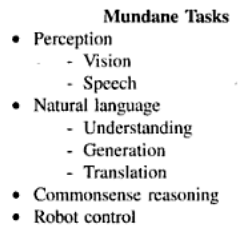
\includegraphics[width=.75\linewidth]{tareas_mundanas}
  \captionof{figure}{Tareas\\mundanas}
  \label{fig:tmundanas}
\end{minipage}%
\begin{minipage}{.33\textwidth}
  \centering
  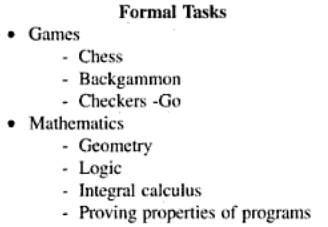
\includegraphics[width=\linewidth]{tareas_formales}
  \captionof{figure}{Tareas\\formales}
  \label{fig:tformales}
\end{minipage}
\begin{minipage}{.33\textwidth}
  \centering
  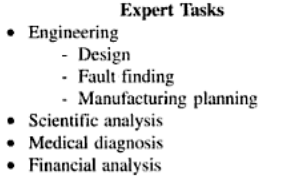
\includegraphics[width=\linewidth]{tareas_expertas}
  \captionof{figure}{Tareas\\expertas}
  \label{fig:texpertas}
\end{minipage}
\end{figure}

En las figuras \ref{fig:tmundanas}, \ref{fig:tformales} y \ref{fig:texpertas} se presenta una lista de tareas propuesta por \cite{rich2009} que hacer referencia a los dominios de las tareas que ataca la inteligencia artificial.



\section{Anexos}
\subsection{Datos Premio Loebner}
\label{sec:an1}
A continuaci\'on se listan los resultados de diferentes a\~nos para el Premio Loebner, extra\'idos de \cite{loebner1}.
\begin{figure}[h]
\centering
\begin{minipage}{.5\textwidth}
  \centering
  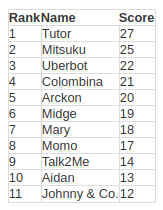
\includegraphics[width=.4\linewidth]{TT2018}
  \captionof{figure}{Resultados 2018}
  \label{fig:tt2018}
\end{minipage}%
\begin{minipage}{.5\textwidth}
  \centering
  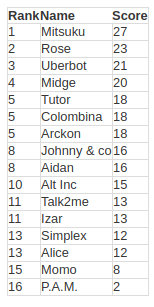
\includegraphics[width=.4\linewidth]{TT2017}
  \captionof{figure}{Resultados 2017}
  \label{fig:tt2017}
\end{minipage}
\end{figure}

\begin{figure}[H]
\centering
\begin{minipage}{.5\textwidth}
  \centering
  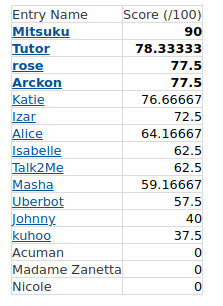
\includegraphics[width=.4\linewidth]{TT2016}
  \captionof{figure}{Resultados 2016}
  \label{fig:tt2016}
\end{minipage}%
\begin{minipage}{.5\textwidth}
  \centering
  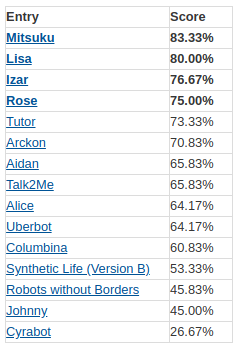
\includegraphics[width=.4\linewidth]{TT2015}
  \captionof{figure}{Resultados 2015}
  \label{fig:tt2015}
\end{minipage}
\end{figure}

\begin{figure}[H]
  \centering
  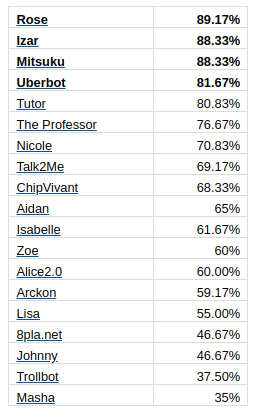
\includegraphics[width=.4\linewidth]{TT2014}
  \caption{Resultados 2014}
  \label{fig:tt2014}
\end{figure}

% ==========Bibliografia===================================

\begin{thebibliography}{99}
	% Item 1
	\bibitem[Russel y Norvig, 2004]{russel}
	\newblock \textsc{Russel, S. J.; Norvig, P.} \textit{Inteligencia Artificial, Un Enfoque Moderno}. Pearson Educaci\'on, S.A., Madrid, 2004, \textsc{ISBN: 84-205-4003-x}
	% Item 2
	\bibitem[Gonz\'alez, 2007]{gonzalez2007} \textsc{Rodrigo Gonz\'alez}. \textit{El test de Turing: dos mitos, un dogma}. Katholieke Universiteit Leuven, 2007, \textsc{doi: 10.4067/S0718-43602007000100003}
	% Item 3
	\bibitem[AISB]{loebner1} \textsc{The Society for the Study of Artificial Intelligence and Simulation of Behaviour}. \textit{Loebner Prize}. AISB. https://www.aisb.org.uk/events/loebner-prize [Consultado el 4 de Septiembre, 2018]
	% Item 4
	\bibitem[VA, 2010]{loebner2} \textsc{Varios autores}. \textit{El test de Turing en su m\'axima competici\'on: Loebner Prize}. System and Software Engineering, 2004. http://www.gtd.es/es/blog/el-test-de-turing-en-su-maxima-competicion-loebner-prize [Consultado el 4 de Septiembre, 2018]
	% Item 5
	\bibitem[Moloney, 2017]{loebner3} \textsc{Charlie Moloney}. \textit{How to win a Turing Test (the Loebner Prize)}. Chatbots Magazine, 2017. https://chatbotsmagazine.com/how-to-win-a-turing-test-the-loebner-prize-3ac2752250f1 [Consultado el 4 de Septiembre, 2018]
	% Item 6
	\bibitem[Cole, 2014]{cole2014} \textsc{David, Cole}.\textit{The Chinese Room Argument}. The Stanford Encyclopedia of Philosophy (Winter 2015 Edition), Edward N. Zalta (ed.), https://plato.stanford.edu/archives/win2015/entries/chinese-room [Consultado el 5 de Septiembre, 2018]
	% Item 7
	\bibitem[Searle, 2009]{searle2009} \textsc{John, Searle}.\textit{Chinese room argument}. Scholarpedia, 4(8):3100. http://dx.doi.org/10.4249/scholarpedia.3100 [Consultado el 5 de Septiembre, 2018]
	% Item 8
	\bibitem[Searle, 1980]{searle1980} \textsc{John, Searle}. \textit{Minds, Brains and Programs}, Behavioral and Brain Sciences, 3: 417-457, http://cogprints.org/7150/1/10.1.1.83.5248.pdf
	% Item 9
	\bibitem[Rich, et al, 2009]{rich2009} \textsc{Elaine, Rich; Kevin, Knight; Shivashankar, B Nair}. \textit{Artificial Intelligence - Third Edition}. McGraw-Hill, 2009. \textsc{isbn-13: 978-0-07-008770-5}
	% Item 10
	\bibitem[Elbot]{elbot}\textsc{Elbot}.  Kiwilogic's Chatterbot. http://www.elbot.com/
	% Item 11
	\bibitem[Tech Insider, 2017]{tideepmind} \textsc{Tech Insider}. \textit{Google's DeepMind AI Just Taught Itself To Walk}. Tech Insider, 2017. https://www.youtube.com/watch?v=gn4nRCC9TwQ [Consultado el 7 de Septiembre, 2018]
	% Item 12
	\bibitem[DeepMind]{deepmind} \textsc{DeepMind}. https://deepmind.com/
	% Item 13
	\bibitem[Jaderberg, et al, 2018]{deepmindquake}\textsc{Max Jaderberg, Wojciech M. Czarnecki, Iain Dunning, Luke Marris Guy Lever, Antonio Garcia Castaneda, Charles Beattie, Neil C. Rabinowitz Ari S. Morcos, Avraham Ruderman, Nicolas Sonnerat, Tim Green, Louise Deason, Joel Z. Leibo, David Silver, Demis Hassabis, Koray Kavukcuoglu, Thore Graepel}. \textit{Human-level performance in first-person multiplayer games with population-based deep reinforcement learning}. DeepMind, London, UK, 2018.
	% Item 14
	\bibitem[Two Minute Papers, 2018]{deepmindquakeresumen}\textsc{Two Minute Papers}. \textit{DeepMind Has A Superhuman Level Quake 3 AI Team}. https://www.youtube.com/watch?v=MvFABFWPBrw [Consultado el 7 de Septiembre, 2018]
	% Item 15
	\bibitem[Watson]{watson}\textsc{IBM}, \textit{Watson}. https://www.ibm.com/watson/ [Consultado el 7 de Septiembre, 2018]
	% Item 16
	\bibitem[Watson Health]{watsononcologia}\textsc{IBM}. \textit{Watson Oncology}. IBM. https://www.ibm.com/watson/health/oncology-and-genomics/genomics/ [Consultado el 7 de Septiembre, 2018]

\end{thebibliography}

\end{document}
